% Sample article using the sbc20 class.
%
% The non-textual content of this file (package loading commands,
% explanatory comments, etc.) was created by Nelson Lago <lago@ime.usp.br>
% and José Viterbo Filho <viterbo@ic.uff.br>. It is licensed under the
% Creative Commons Attribution International Licence, v4.0 (CC-BY 4.0)
% https://creativecommons.org/licenses/by/4.0/
%
% Using the non-textual content of this file as a template to produce
% your own document without further attribution to the authors above
% is permitted and encouraged.
%
% charset: utf-8 ãàáâéêíõóôúç ÃÀÁÂÉÊÍÕÓÔÚÇ

% The last language is the main language of the document.
\documentclass[english,notblind]{sbc20}


%%%%%%%%%%%%%%%%%%%%%%%%%%%%%%%%%%%%%%%%%%%%%%%%%%%%%%%%%%%%%%%%%%%%%%%%%%%%%%%%
%%%%%%%%%%%%%%%%%%%%%%%%%%%%%%%%%% PACKAGES %%%%%%%%%%%%%%%%%%%%%%%%%%%%%%%%%%%%
%%%%%%%%%%%%%%%%%%%%%%%%%%%%%%%%%%%%%%%%%%%%%%%%%%%%%%%%%%%%%%%%%%%%%%%%%%%%%%%%

% Basics
\usepackage{verbatim}  % support for unformatted text, almost mandatory
\usepackage{graphicx}  % support for figures etc., almost mandatory
\usepackage{array}     % extra table features, almost mandatory
\usepackage{pbalance}  % equal heights in last page columns (demands additional LaTeX passes)
\usepackage{mathtools} % extra visual tweaks/features for math, read the docs

% Table improvements
\usepackage{booktabs}  % better table aesthetics, recommended, read the docs
\usepackage{multirow}  % table cells that span over multiple rows
\usepackage{makecell}  % better table headings / cells with linebreaks inside
\usepackage{dcolumn}   % align numeric columns on the decimal separator (siunitx also offers this)
\usepackage{longtable} % multi-page tables
\usepackage{threeparttable} % tables with "footnotes"
%\usepackage{colortbl}  % colored table cells
%\usepackage{csvsimple} % load a csv file and format as table

% Extra features for floats
\usepackage{rotating}   % \sidewaystable, \sidewaysfigure, and other rotation commands
\usepackage[above,below]{placeins} % manually control float placement, read the docs
\usepackage{subcaption} % subfigures (side by side) with subcaptions (pkg subfigure is deprecated)
\usepackage{adjustbox}  % resize, clip etc. for any material, not only floats

% Source code syntax highlighting
%\usepackage{listings} % good and simple
%\usepackage{minted}   % excellent, but depends on pygments (python, free software)

%\usepackage{siunitx} % Numbers: units, scientific notation, better presentation for large numbers

%\usepackage{pdfcomment} % useful in the writing/reviewing phase


%%%%%%%%%%%%%%%%%%%%%%%%%%%%%%%%%%%%%%%%%%%%%%%%%%%%%%%%%%%%%%%%%%%%%%%%%%%%%%%%
%%%%%%%%%%%%%%%%%%%%%%%%%%%%%%% ARTICLE METADATA %%%%%%%%%%%%%%%%%%%%%%%%%%%%%%%
%%%%%%%%%%%%%%%%%%%%%%%%%%%%%%%%%%%%%%%%%%%%%%%%%%%%%%%%%%%%%%%%%%%%%%%%%%%%%%%%

% With bibLaTeX, the bibliographic databases are defined in the preamble.
% Call \addbibresource multiple times to use more than one file.
\addbibresource{bibliografia.bib}

\metadata
  {
    pubname={Simpósio Brasileiro de Alguma Área de Pesquisa},
    pubacron={SBAAP},
    idjems={XXX},
    copyrightyear=2025,
    category={Full Paper},
    bibstyle=sbc20,
    %bibstyle=sbc20-authordate,
    %nocolorlinks, % disable colored hyperlinks, for B&W printing
  }
  
\title
  {
    mainlanguagetitle={Example of use of the SBC template for papers written in English to be published in SOL event proceedings},
  }

% These are used in the headers and are optional; if not
% defined, the complete title and all authors will appear
\shortauthor{Viterbo et al. 2025}
\shorttitle{Template for SOL papers written in English}
  
\author
  {
    % special chars in email addresses (%, _, $, &, #, ~ etc.)
    % are ok if the whole address is within braces
    email=viterbo@ic.uff.br,
    orcid=0000-0002-0339-6624, % without "http" etc.
    institutionID=UFF,
    country=Brasil,
    firstName=José,
    lastName=Viterbo 
  }
  

\author
  {
    email=lago@ime.usp.br,
    orcid=0000-0002-4306-8078,
    % institutionID may be called multiple times or include
    % multiple items separated by commas (within braces)
    institutionID={USP,UPa},
    % institutionID={usp,upa},
    country=Brasil,
    firstName=Nelson,
    middleName=Silva,
    lastName=Lago
  }
  

  \author
  {
    email=rmvieira@inf.ufrgs.br,
    orcid=0009-0009-1113-0867,
    institutionID={UFRGS},
    country=Brasil,
    firstName=Raphael,
    middleName=Malinski,
    lastName=Vieira
  }


\author
  {
    email=granville@inf.ufrgs.br,
    orcid=0000-0001-8956-8660,
    institutionID=UFRGS,
    country=Brasil,
    firstName=Lisandro,
    lastName=Granville
  }

  

\institution{UFF}{Universidade Federal Fluminense}
\institution{UFMT}{Universidade Federal de Mato Grosso}
\institution{UFPR}{Universidade Federal do Paraná}

\institution{USP}
  {Universidade de São Paulo}

\institution{UPa}
  {Universidade de Pasárgada}

\institution{UFRGS}
  {Universidade Federal do Rio Grande do Sul}

% This space can be used to detail/complement information about authors and their affiliations. This item is optional...
\extraAffiliationsLast{José Viterbo is an Associate Professor at the Institute of Computing at UFF and Director of Publications at SBC. Nelson Lago is a researcher at the Center for Competence in Free Software at USP and at the School of Arts, Sciences and Humanities at UPa. Raphael Malinski Vieira is a student of the Bachelor's degree in Computer Science at UFRGS. Lisandro Granville is a Full Professor at the Institute of Informatics at UFRGS and Financial Director of SBC.}

\abstract
  {
    This text, formatted as a scientific article, aims to present the new SBC paper template, describing its main features and explaining how it should be used. This version, more specifically, should be used exclusively for articles written in English that will be published in any event proceeding series at SBC OpenLib. The abstract in Portuguese, as you can see in this example, must be before the abstract in English and must have between 500 and 750 words.
  }

\keywords{Proceedings \sep Template \sep SBC OpenLib \sep Indexing}

\palavraschave{}


% These are all optional; they appear at the end of the document

\contributeinfo{JV elaborou a primeira versão do template e os textos explicativos. NSL aprimorou o modelo. LG propôs a inclusão de metadados no PDF gerado e RMV implementou esta proposta.}

\acknowledgements{Agradecimentos a colegas, colaboradores etc. Essa declaração é opcional, se não houver nenhum agradecimento, pode ser deixada em branco}

\funding{Indicação de agências financiadoras etc. Essa declaração é opcional, se não houver nenhum financiamento, pode ser deixada em branco.}

\datainfo{
  Links para dados  e materiais adicionais disponíveis, como código, página do projeto etc. Essa declaração é obrigatória. Se os dados não forem disponibilizados previamente, pode-se declarar: ``Os dados e/ou materiais adicionais poderão ser disponibilizados mediante solicitação.''
}

\furtherinfo{Informações adicionais relevantes, como, por exemplo, a aprovação em comitê de ética ou o uso de ferramentas de IA generativa no desenvolvimento do artigo. Essa declaração é opcional, se não houver nada a ser acrescentado, pode ser deixada em branco}

\SBCprintbibliography
%%%%%%%%%%%%%%%%%%%%%%%%%%%%%%%%%%%%%%%%%%%%%%%%%%%%%%%%%%%%%%%%%%%%%%%%%%%%%%%%
%%%%%%%%%%%%%%%%%%%%%%%%%%%%%%%%% BEGIN TEXT %%%%%%%%%%%%%%%%%%%%%%%%%%%%%%%%%%%
%%%%%%%%%%%%%%%%%%%%%%%%%%%%%%%%%%%%%%%%%%%%%%%%%%%%%%%%%%%%%%%%%%%%%%%%%%%%%%%%

\begin{document}

\maketitle

\section{Introduction}
\label{sec:intro}

The SBC OpenLib\footnote{\url{sol.sbc.org.br}} is the new digital library of the Brazilian Computer Society (SBC), and its main objective is to facilitate access to specialized information on Computing. Its collection consists of conference proceedings, nationally and internationally renowned journals, books and chapters resulting from scientific production carried out within the scope of the SBC, offering open access to all publications.

This text, in scientific article format, aims to present the new model for SBC articles, describing its main characteristics, explaining how it should be used and presenting practical examples. This version, more specifically, should be used as a reference exclusively for the preparation of articles written in Portuguese that will be published in some series of conference proceedings in the SBC OpenLib.

This same model should be adopted for both full and short articles, with event organizers being responsible for defining the maximum and minimum limits for the number of pages in each case. The Table~\ref{tab:equivalence} shows the correspondence of the number of pages between the new model and the previous SBC article template, in order to guide event organizers in the transition between models.

% TODO: Mudamos o tamanho da fonte, é preciso recalcular isto! -> fiz um experimento com blind text, a proporção foi 9:6, ou seja, esta tabela parece ok.
\begin{table}[!hb]
\centering
\begin{tabular}{@{}cc@{}}
\toprule
Previous template (2005) & New template (2025) \\
\midrule
 4  & 3 \\
 6  & 4 \\
 8  & 6 \\
 12  & 8 \\
\bottomrule
\end{tabular}
\caption{Page count correspondence considering the previous SBC article template, released in 2025, and the new template, released in 2025.\label{tab:equivalence}}
\end{table}

Figure~\ref{fig:page-layout} presents the \emph{page layout}. The following sections provide detailed information about each part of the model. In Section 2, we describe the details of the article header. In Section 3, we describe the details of the article opening. In Section 4, we describe the sections and subsections of the paper. In Section 5, we describe the use of tables, figures, and algorithms in the paper. In Section 6, we discuss the forms of citations and the inclusion of references.

% TODO: if there will not be a footer, remove it from the figure
\begin{figure}
  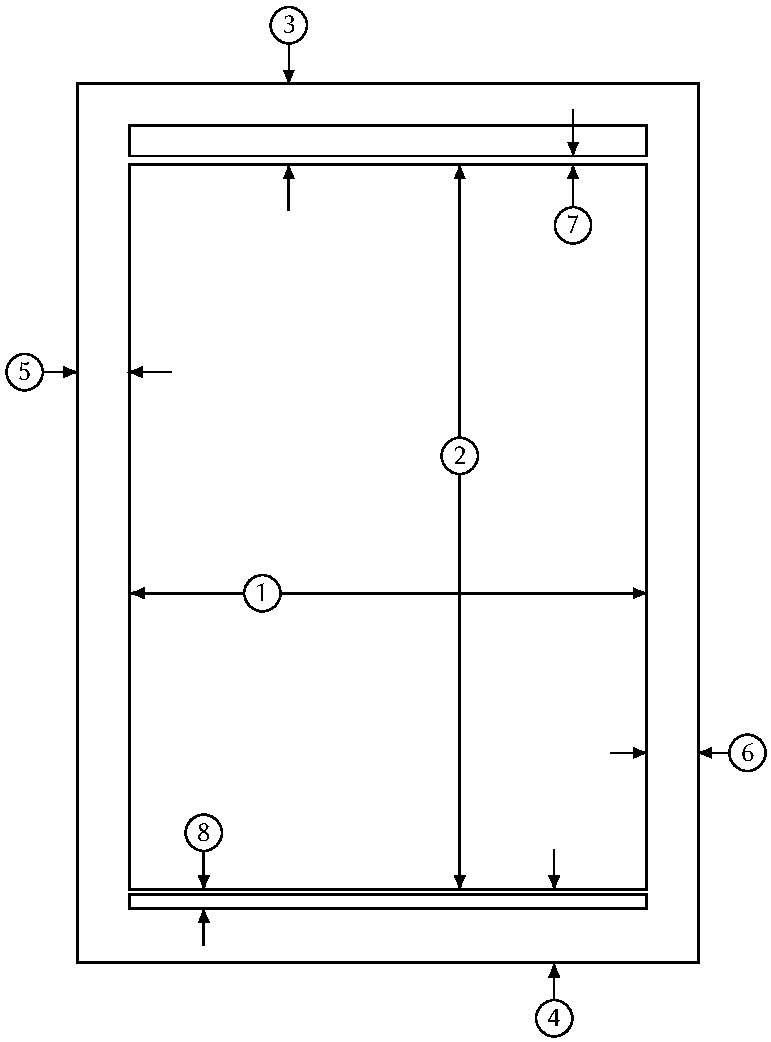
\includegraphics[width=\columnwidth]{figures/page-layout}
  \caption{\emph{Layout} da página. O tamanho é A4 (210\,x\,297\,mm);
  a mancha de texto (1 e 2) mede 175\,x\,246\,mm; a margem superior
  (3) é 26\,mm e a margem inferior (4) é 23\,mm; as margens esquerda
  (5) e direita (6) medem 17,5\,mm; o espaço entre o cabeçalho e o
  texto (7) é 10\,pt; a distância entre o final do texto e o final do
  rodapé (8) é 18\,pt; o espaço entre as colunas (não mostrado) é
  18\,pt.\label{fig:page-layout}}
\end{figure}

\section{Cabeçalho}

O cabeçalho do artigo tem duas variações, uma para a primeira página e outra para as páginas seguintes. Ambas são descritas nas subseções a seguir.

\subsection{Cabeçalho da Primeira Página}

Na primeira página, o cabeçalho apresenta o título da série e o ano da edição em uma primeira linha. A segunda linha traz a descrição da licença de publicação, que para os eventos que disponibilizam seus artigos na SBC OpenLib corresponde à licença CC BY-NC 4.0. Os autores devem preencher a informação do título da série, acrônimo do evento e ano do evento nos campos \textit{jtitle}, \textit{jid} e \textit{jyear}, respectivamente. A informação sobre a licença deve constar do campo \textit{copyrightstatement}.

\subsection{Cabeçalho da Página 2 em diante}

A partir da página 2, o cabeçalho apresenta o título resumido à esquerda e a lista de autores resumida à direita. O título abreviado do artigo e a lista abreviada de autores devem ser preenchidos em \textit{shorttitle} e \textit{shortauthors}, respectivamente.

\section{Abertura}

O preâmbulo do artigo contém os principais metadados que descrevem o artigo: o título, o resumo e as palavras-chave, tanto em inglês, quanto em português.

\subsection{Título}

\subsection{Autores}

\section{Bibliografia}

Citações e referências bibliográficas devem seguir o formato definido pela ABNT (NBR\,10520, versão 2002 e NBR\,6023 versão 2002 ou, preferencialmente, 2018). Os organizadores de cada evento definem se as citações seguirão o formato numérico ou autor-data. Observe que:

\begin{itemize}
  \item Endereços web (URLs) não são colocados entre ``<\,>'' (esse é o padrão na versão 2018 da NBR\,6023)
  \item ``In'' e ``et al.'' são formatados em itálico (esse é o padrão na versão 2018 da NBR\,6023)
  \item No formato numérico, os sobrenomes não são grafados em caixa alta
  \item No formato autor-data, usa-se versalete para os sobrenomes (com a primeira letra maiúscula)
\end{itemize}

\section{Outros exemplos}

Esta classe é baseada na classe \texttt{article} e, portanto, os comandos usuais de \LaTeX, como \textsf{\textbackslash{}verse}, \textsf{\textbackslash{}quotation} etc. podem ser usados normalmente:

\begin{verse}
Batatinha quando nasce\\
Espalha a rama pelo chão

A menina quando dorme\\
Põe a mão no coração
\end{verse}

\begin{quotation}
\itshape
Algum tempo hesitei se devia abrir estas memórias pelo princípio ou
pelo fim, isto é, se poria em primeiro lugar o meu nascimento ou a
minha morte. Suposto o uso vulgar seja começar pelo nascimento,
duas considerações me levaram a adotar diferente método: a
primeira é que eu não sou propriamente um autor defunto, mas um
defunto autor, para quem a campa foi outro berço; a segunda é que
o escrito ficaria assim mais galante e mais novo. Moisés, que também
contou a sua morte, não a pôs no intróito, mas no cabo: diferença
radical entre este livro e o Pentateuco.
\end{quotation}

Equações de segundo grau (Equação \ref{eq:2grau}) são estudadas no ensino
médio. As raízes de uma equação de segundo grau podem ser encontradas
por~\eqref{eq:bhaskara} --- a fórmula de Bháskara. O valor do discriminante
$\Delta$ (Equação \ref{eq:delta}) determina se a equação tem zero, uma ou
duas raízes reais distintas.

\begin{equation}
  \label{eq:2grau}
  ax^2+bx+c=y \quad \forall x \in \mathbb{R}
\end{equation}

\begin{gather}
  \label{eq:bhaskara}
    y=0 \Leftrightarrow x=\frac{-b \pm \sqrt{\Delta}}{2a}
    \Leftrightarrow x \text{ é raiz da equação}\\
  \label{eq:delta}
    \Delta\enspace(\mathit{delta}) = b^2-4ac
\end{gather}

\begin{figure}
  \centering
  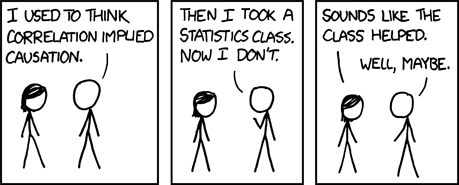
\includegraphics[width=\columnwidth]{figures/xkcd_552_correlation}
   \caption{A bitmap figure (from \url{xkcd.com/552}).\label{fig:xkcd-correlation}}
\end{figure}

\begin{figure*}[b]
  \centering
  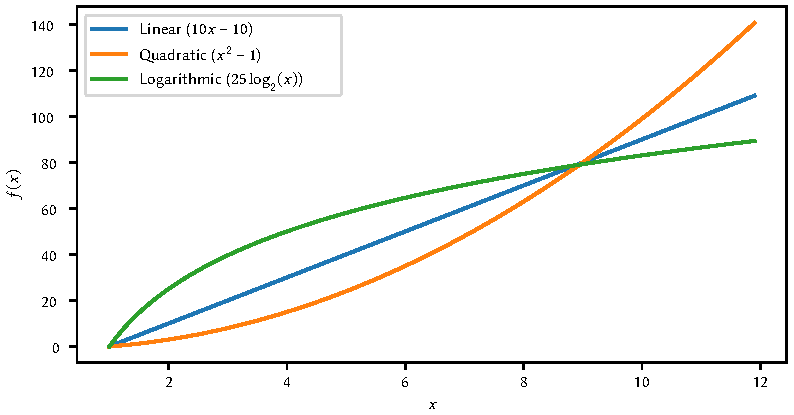
\includegraphics{figures/graph-functions}
  \caption{A vector figure spanning both text columns.\label{fig:graph-functions}}
\end{figure*}

Imagens vetoriais (como diagramas e gráficos, a exemplo das Figuras~\ref{fig:page-layout}~e~\ref{fig:graph-functions}) \emph{não} devem ser convertidas para \emph{bitmaps}, mas sim mantidas em algum formato vetorial, como PDF. Imagens não-vetoriais com cores predominantemente sólidas (como a Figura~\ref{fig:xkcd-correlation}) devem ser convertidas para o formato PNG e imagens fotográficas ou com texturas devem ser convertidas para o formato JPEG. Uma figura ou tabela muito grande (Figura~\ref{fig:graph-functions}, Tabela~\ref{tab:form}) pode excepcionalmente ocupar a largura das duas colunas de texto, mas apenas no início ou no final da página. Todas as figuras e tabelas devem ser acompanhadas das respectivas legendas explicativas numeradas logo abaixo delas.

\begin{table*}
  \centering
  \newcolumntype{M}[1]{>{\centering}m{#1\textwidth}}
  \begin{threeparttable}
    \begin{tabular}{|M{0.265}|M{0.073}|M{0.084}|M{0.073}|M{0.073}|M{0.08}|M{0.082}|M{0.067}|}
        \hline
      \textbf{Experimento número:} & \multicolumn{2}{c|}{1} & \multicolumn{4}{c|}{\textbf{Data:}} & jan 2017
        \tabularnewline \hline
      \textbf{Título:} & \multicolumn{7}{c|}{Medições iniciais}
        \tabularnewline \hline
      \textbf{Tipo:} & \multicolumn{7}{c|}{Levantamento quantitativo}
        \tabularnewline \hline \hline
      \textbf{Locais}          & São Paulo & Rio de Janeiro & Porto Alegre & Recife & Manaus & Brasília & Rio Branco
        \tabularnewline \hline
      \textbf{Valores obtidos} & 0.2       & 0.3            & 0.2          & 0.7    & 0.5    & 0.1      & 0.4\tnote{a}
        \tabularnewline \hline
    \end{tabular}
    \begin{tablenotes}
      \item[a] This is an example of table footnote with a reference
      \item This is an example of table footnote without a reference
    \end{tablenotes}
    \caption{A table spanning both text columns.\label{tab:form}}
  \end{threeparttable}
\end{table*}

\section{Conclusion}

\begin{itemize}
  \item @Book: \cite{Knuth:96}.

  \item @Article (em periódico): \cite{floats2014}.

  \item @InProceedings (ou @Conference): \cite{alves03:simi}.

  \item @InCollection (capítulo de livro ou coletânea): \cite{bobaoglu93:concepts}.

  \item @PhdThesis: \cite{garcia01:PhD}.

  \item @MastersThesis: \cite{schmidt03:MSc}.

  \item @Techreport: \cite{alvisi99:analysisCIC}.

  \item @Manual: \cite{biblatex}.

  \item @Misc: \cite{gridftp}.

  \item @Online (para referência a artigo \emph{online}): \cite{fowler04:designDead}.

  \item @Online (para referência a página web): \cite{FSF:GNU-GPL}.

  \item @article (para referência a página web): \cite{alon09:how}.
  
\end{itemize}


%%%%%%%%%%%%%%%%%%%%%%%%%%%%%%%%%%%%%%%%%%%%%%%%%%%%%%%%%%%%%%%%%%%%%%%%%%%%%%%%
%%%%%%%%%%%%%%%%%%%%%%%%%%%%%%%%% BIBLIOGRAPHY %%%%%%%%%%%%%%%%%%%%%%%%%%%%%%%%%
%%%%%%%%%%%%%%%%%%%%%%%%%%%%%%%%%%%%%%%%%%%%%%%%%%%%%%%%%%%%%%%%%%%%%%%%%%%%%%%%

\end{document}
